\documentclass[twoside]{book}

% Packages required by doxygen
\usepackage{fixltx2e}
\usepackage{calc}
\usepackage{doxygen}
\usepackage[export]{adjustbox} % also loads graphicx
\usepackage{graphicx}
\usepackage[utf8]{inputenc}
\usepackage{makeidx}
\usepackage{multicol}
\usepackage{multirow}
\PassOptionsToPackage{warn}{textcomp}
\usepackage{textcomp}
\usepackage[nointegrals]{wasysym}
\usepackage[table]{xcolor}

% Font selection
\usepackage[T1]{fontenc}
\usepackage[scaled=.90]{helvet}
\usepackage{courier}
\usepackage{amssymb}
\usepackage{sectsty}
\renewcommand{\familydefault}{\sfdefault}
\allsectionsfont{%
  \fontseries{bc}\selectfont%
  \color{darkgray}%
}
\renewcommand{\DoxyLabelFont}{%
  \fontseries{bc}\selectfont%
  \color{darkgray}%
}
\newcommand{\+}{\discretionary{\mbox{\scriptsize$\hookleftarrow$}}{}{}}

% Page & text layout
\usepackage{geometry}
\geometry{%
  a4paper,%
  top=2.5cm,%
  bottom=2.5cm,%
  left=2.5cm,%
  right=2.5cm%
}
\tolerance=750
\hfuzz=15pt
\hbadness=750
\setlength{\emergencystretch}{15pt}
\setlength{\parindent}{0cm}
\setlength{\parskip}{3ex plus 2ex minus 2ex}
\makeatletter
\renewcommand{\paragraph}{%
  \@startsection{paragraph}{4}{0ex}{-1.0ex}{1.0ex}{%
    \normalfont\normalsize\bfseries\SS@parafont%
  }%
}
\renewcommand{\subparagraph}{%
  \@startsection{subparagraph}{5}{0ex}{-1.0ex}{1.0ex}{%
    \normalfont\normalsize\bfseries\SS@subparafont%
  }%
}
\makeatother

% Headers & footers
\usepackage{fancyhdr}
\pagestyle{fancyplain}
\fancyhead[LE]{\fancyplain{}{\bfseries\thepage}}
\fancyhead[CE]{\fancyplain{}{}}
\fancyhead[RE]{\fancyplain{}{\bfseries\leftmark}}
\fancyhead[LO]{\fancyplain{}{\bfseries\rightmark}}
\fancyhead[CO]{\fancyplain{}{}}
\fancyhead[RO]{\fancyplain{}{\bfseries\thepage}}
\fancyfoot[LE]{\fancyplain{}{}}
\fancyfoot[CE]{\fancyplain{}{}}
\fancyfoot[RE]{\fancyplain{}{\bfseries\scriptsize Generated by Doxygen }}
\fancyfoot[LO]{\fancyplain{}{\bfseries\scriptsize Generated by Doxygen }}
\fancyfoot[CO]{\fancyplain{}{}}
\fancyfoot[RO]{\fancyplain{}{}}
\renewcommand{\footrulewidth}{0.4pt}
\renewcommand{\chaptermark}[1]{%
  \markboth{#1}{}%
}
\renewcommand{\sectionmark}[1]{%
  \markright{\thesection\ #1}%
}

% Indices & bibliography
\usepackage{natbib}
\usepackage[titles]{tocloft}
\setcounter{tocdepth}{3}
\setcounter{secnumdepth}{5}
\makeindex

% Hyperlinks (required, but should be loaded last)
\usepackage{ifpdf}
\ifpdf
  \usepackage[pdftex,pagebackref=true]{hyperref}
\else
  \usepackage[ps2pdf,pagebackref=true]{hyperref}
\fi
\hypersetup{%
  colorlinks=true,%
  linkcolor=blue,%
  citecolor=blue,%
  unicode%
}

% Custom commands
\newcommand{\clearemptydoublepage}{%
  \newpage{\pagestyle{empty}\cleardoublepage}%
}

\usepackage{caption}
\captionsetup{labelsep=space,justification=centering,font={bf},singlelinecheck=off,skip=4pt,position=top}

%===== C O N T E N T S =====

\begin{document}

% Titlepage & ToC
\hypersetup{pageanchor=false,
             bookmarksnumbered=true,
             pdfencoding=unicode
            }
\pagenumbering{roman}
\begin{titlepage}
\vspace*{7cm}
\begin{center}%
{\Large Transit Network Model }\\
\vspace*{1cm}
{\large Generated by Doxygen 1.8.11}\\
\end{center}
\end{titlepage}
\clearemptydoublepage
\tableofcontents
\clearemptydoublepage
\pagenumbering{arabic}
\hypersetup{pageanchor=true}

%--- Begin generated contents ---
\chapter{Main Page}
\label{index}\hypertarget{index}{}A realtime model of a public transport network.

An program which runs indefinitely, modeling the realtime state of all vehicles in the transit network. These are in turn used to model the realtime state of the network itself (road speeds), and finally arrival time predictions made for each vehicle/stop combination.


\begin{DoxyItemize}
\item \hyperlink{transit__network__model_8cpp}{transit\+\_\+network\+\_\+model.\+cpp} 
\end{DoxyItemize}
\chapter{Transit Network Model}
\label{md_README}
\hypertarget{md_README}{}
Three parts, running in real time\+:
\begin{DoxyEnumerate}
\item particle filter for vehicle location and speed
\item Kalman filter for transit road network state (speed)
\item travel-\/ and arrival-\/time predictions for each vehicle/stop combination in the network
\end{DoxyEnumerate}

\subsubsection*{1. Particle Filter}

{\bfseries IN}\+: G\+T\+FS realtime protobuf feed

{\bfseries O\+UT}\+: (updated) vehicle objects with updated particle states

\subsubsection*{2. Kalman filter}

{\bfseries IN}\+: particle filter state estimates, road state at time {\ttfamily now -\/ delta}

{\bfseries O\+UT}\+: road state at time {\ttfamily now}

\subsubsection*{3. Predictions}

{\bfseries IN}\+: particle filter state estimates, road state estimates

{\bfseries O\+UT}\+: E\+TA to remaining stops along route



 \subsection*{Dependencies}


\begin{DoxyItemize}
\item C\+Make
\item (optional) Doxygen (for making the Documentation)
\item (optional) https\+://github.com/google/protobuf/blob/master/src/\+R\+E\+A\+D\+M\+E.\+md \char`\"{}\+Google protobuf compiler `protoc`\char`\"{}
\end{DoxyItemize}

\subsection*{To-\/do}


\begin{DoxyItemize}
\item Application to run indefinitely
\item Use a {\ttfamily Vehicle} object concept with
\begin{DoxyItemize}
\item {\ttfamily vector$<$Particle$>$ (N)}
\item {\ttfamily void update (gtfs\+::\+Vehicle\+Position, gtfs\+::\+Trip\+Update)}\+: adjust the position, arrival/departure times etc, trigger particle transitions
\item {\ttfamily void resample (N)}\+: perform particle filter weighted resample
\item properties {\ttfamily vehicle\+\_\+id}, {\ttfamily timestamp}, {\ttfamily trip\+\_\+id}, {\ttfamily route\+\_\+id}, {\ttfamily position}, {\ttfamily stop\+\_\+sequence}, {\ttfamily arrival\+\_\+time}, {\ttfamily departure\+\_\+time}
\end{DoxyItemize}
\item And the particles work in memory only
\begin{DoxyItemize}
\item {\ttfamily Particle}
\begin{DoxyItemize}
\item {\ttfamily void initialize ()}
\item {\ttfamily void transition ()}
\item {\ttfamily void calc\+\_\+likelihood ()}\+: uses parent Vehicle
\item {\ttfamily void calc\+\_\+weight ()}
\item properties {\ttfamily distance}, {\ttfamily velocity}, {\ttfamily stop\+\_\+index}, {\ttfamily arrival\+\_\+time}, {\ttfamily departure\+\_\+time}, {\ttfamily segment\+\_\+index}, {\ttfamily queue\+\_\+time}, {\ttfamily begin\+\_\+time}, {\ttfamily likelihood}, {\ttfamily weight}
\end{DoxyItemize}
\end{DoxyItemize}
\item Similar concept for network route segments
\begin{DoxyItemize}
\item {\ttfamily Segment}
\begin{DoxyItemize}
\item {\ttfamily vector$<$Path$>$ shape}\+: the G\+PS coordinates and cumulative distance of segment shape
\item {\ttfamily double speed}
\item {\ttfamily void update ()}\+: perform Kalman filter update, using particle summaries (?)
\end{DoxyItemize}
\end{DoxyItemize}
\item The G\+T\+FS information can either be
\begin{DoxyItemize}
\item loaded into an S\+Q\+Lite database, or
\item loaded into a M\+E\+M\+O\+RY table via My\+S\+QL
\end{DoxyItemize}
\item Vehicle state summaries can be written to a file (?)
\item Making information available (via server) -\/ road segment speeds + arrival time predictions
\begin{DoxyItemize}
\item database (with no foreign key checks, and no transaction?)
\end{DoxyItemize}
\end{DoxyItemize}

(?) best way of collecting vehicle/segment data
\begin{DoxyItemize}
\item sequentially append speed estimates to {\ttfamily Segment}, then periodically update and clear?
\item write to file? (makes keeping history easier?)
\end{DoxyItemize}

\subsection*{Project Structure}


\begin{DoxyItemize}
\item {\ttfamily bin}
\begin{DoxyItemize}
\item {\ttfamily transit\+\_\+network\+\_\+model}\+: the application that\textquotesingle{}ll run \textquotesingle{}infinitely\textquotesingle{}
\item {\ttfamily load\+\_\+gtfs}\+: this will load G\+T\+FS when updates released, and do the segmentation
\end{DoxyItemize}
\item {\ttfamily src}
\begin{DoxyItemize}
\item {\ttfamily \hyperlink{transit__network__model_8cpp}{transit\+\_\+network\+\_\+model.\+cpp}}\+: mostly just a wrapper for {\ttfamily while (T\+R\+UE) \{ ... \}}
\item {\ttfamily laod\+\_\+gtfs.\+cpp}
\end{DoxyItemize}
\item {\ttfamily include}
\begin{DoxyItemize}
\item {\ttfamily gtfs}\+: descriptions of the gtfs objects (??)
\begin{DoxyItemize}
\item {\ttfamily \hyperlink{classgtfs_1_1Vehicle}{gtfs\+::\+Vehicle}} a vehicle object
\item {\ttfamily \hyperlink{classgtfs_1_1Particle}{gtfs\+::\+Particle}}
\end{DoxyItemize}
\item {\ttfamily gps}\+: methods for G\+PS coordinates (distance, etc)
\item {\ttfamily particle\+\_\+filter}\+: the particle filter model
\item {\ttfamily kalman\+\_\+filter}\+: the Kalman filter model
\item {\ttfamily segmentation}\+: the segmentation algorithm for (new) segments
\item {\ttfamily database}\+: any database methods (connection, S\+E\+L\+E\+CT, I\+N\+S\+E\+RT, etc)
\end{DoxyItemize}
\item {\ttfamily lib}
\begin{DoxyItemize}
\item {\ttfamily gtfsrealtime.\+proto}\+: the schema for G\+T\+FS protobuf feed 
\end{DoxyItemize}
\end{DoxyItemize}
\chapter{Namespace Index}
\section{Namespace List}
Here is a list of all documented namespaces with brief descriptions\+:\begin{DoxyCompactList}
\item\contentsline{section}{\hyperlink{namespacegps}{gps} }{\pageref{namespacegps}}{}
\item\contentsline{section}{\hyperlink{namespacegtfs}{gtfs} }{\pageref{namespacegtfs}}{}
\item\contentsline{section}{\hyperlink{namespacenlohmann}{nlohmann} \\*Namespace for Niels Lohmann }{\pageref{namespacenlohmann}}{}
\item\contentsline{section}{\hyperlink{namespacenlohmann_1_1detail}{nlohmann\+::detail} \\*Unnamed namespace with internal helper functions }{\pageref{namespacenlohmann_1_1detail}}{}
\item\contentsline{section}{\hyperlink{namespacesampling}{sampling} }{\pageref{namespacesampling}}{}
\end{DoxyCompactList}

\chapter{Class Index}
\section{Class List}
Here are the classes, structs, unions and interfaces with brief descriptions\+:\begin{DoxyCompactList}
\item\contentsline{section}{\hyperlink{structnlohmann_1_1adl__serializer}{nlohmann\+::adl\+\_\+serializer$<$ typename, typename $>$} \\*Default J\+S\+O\+N\+Serializer template argument }{\pageref{structnlohmann_1_1adl__serializer}}{}
\item\contentsline{section}{\hyperlink{classnlohmann_1_1basic__json}{nlohmann\+::basic\+\_\+json$<$ Object\+Type, Array\+Type, String\+Type, Boolean\+Type, Number\+Integer\+Type, Number\+Unsigned\+Type, Number\+Float\+Type, Allocator\+Type, J\+S\+O\+N\+Serializer $>$} \\*Class to store J\+S\+ON values }{\pageref{classnlohmann_1_1basic__json}}{}
\item\contentsline{section}{\hyperlink{structnlohmann_1_1detail_1_1conjunction}{nlohmann\+::detail\+::conjunction$<$... $>$} }{\pageref{structnlohmann_1_1detail_1_1conjunction}}{}
\item\contentsline{section}{\hyperlink{structnlohmann_1_1detail_1_1conjunction_3_01B1_01_4}{nlohmann\+::detail\+::conjunction$<$ B1 $>$} }{\pageref{structnlohmann_1_1detail_1_1conjunction_3_01B1_01_4}}{}
\item\contentsline{section}{\hyperlink{structnlohmann_1_1detail_1_1conjunction_3_01B1_00_01Bn_8_8_8_01_4}{nlohmann\+::detail\+::conjunction$<$ B1, Bn... $>$} }{\pageref{structnlohmann_1_1detail_1_1conjunction_3_01B1_00_01Bn_8_8_8_01_4}}{}
\item\contentsline{section}{\hyperlink{classgps_1_1Coord}{gps\+::\+Coord} }{\pageref{classgps_1_1Coord}}{}
\item\contentsline{section}{\hyperlink{classsampling_1_1exponential}{sampling\+::exponential} }{\pageref{classsampling_1_1exponential}}{}
\item\contentsline{section}{\hyperlink{structnlohmann_1_1detail_1_1external__constructor}{nlohmann\+::detail\+::external\+\_\+constructor$<$ value\+\_\+t $>$} }{\pageref{structnlohmann_1_1detail_1_1external__constructor}}{}
\item\contentsline{section}{\hyperlink{structnlohmann_1_1detail_1_1external__constructor_3_01value__t_1_1array_01_4}{nlohmann\+::detail\+::external\+\_\+constructor$<$ value\+\_\+t\+::array $>$} }{\pageref{structnlohmann_1_1detail_1_1external__constructor_3_01value__t_1_1array_01_4}}{}
\item\contentsline{section}{\hyperlink{structnlohmann_1_1detail_1_1external__constructor_3_01value__t_1_1boolean_01_4}{nlohmann\+::detail\+::external\+\_\+constructor$<$ value\+\_\+t\+::boolean $>$} }{\pageref{structnlohmann_1_1detail_1_1external__constructor_3_01value__t_1_1boolean_01_4}}{}
\item\contentsline{section}{\hyperlink{structnlohmann_1_1detail_1_1external__constructor_3_01value__t_1_1number__float_01_4}{nlohmann\+::detail\+::external\+\_\+constructor$<$ value\+\_\+t\+::number\+\_\+float $>$} }{\pageref{structnlohmann_1_1detail_1_1external__constructor_3_01value__t_1_1number__float_01_4}}{}
\item\contentsline{section}{\hyperlink{structnlohmann_1_1detail_1_1external__constructor_3_01value__t_1_1number__integer_01_4}{nlohmann\+::detail\+::external\+\_\+constructor$<$ value\+\_\+t\+::number\+\_\+integer $>$} }{\pageref{structnlohmann_1_1detail_1_1external__constructor_3_01value__t_1_1number__integer_01_4}}{}
\item\contentsline{section}{\hyperlink{structnlohmann_1_1detail_1_1external__constructor_3_01value__t_1_1number__unsigned_01_4}{nlohmann\+::detail\+::external\+\_\+constructor$<$ value\+\_\+t\+::number\+\_\+unsigned $>$} }{\pageref{structnlohmann_1_1detail_1_1external__constructor_3_01value__t_1_1number__unsigned_01_4}}{}
\item\contentsline{section}{\hyperlink{structnlohmann_1_1detail_1_1external__constructor_3_01value__t_1_1object_01_4}{nlohmann\+::detail\+::external\+\_\+constructor$<$ value\+\_\+t\+::object $>$} }{\pageref{structnlohmann_1_1detail_1_1external__constructor_3_01value__t_1_1object_01_4}}{}
\item\contentsline{section}{\hyperlink{structnlohmann_1_1detail_1_1external__constructor_3_01value__t_1_1string_01_4}{nlohmann\+::detail\+::external\+\_\+constructor$<$ value\+\_\+t\+::string $>$} }{\pageref{structnlohmann_1_1detail_1_1external__constructor_3_01value__t_1_1string_01_4}}{}
\item\contentsline{section}{\hyperlink{structnlohmann_1_1detail_1_1from__json__fn}{nlohmann\+::detail\+::from\+\_\+json\+\_\+fn} }{\pageref{structnlohmann_1_1detail_1_1from__json__fn}}{}
\item\contentsline{section}{\hyperlink{classgtfs_1_1GTFS}{gtfs\+::\+G\+T\+FS} }{\pageref{classgtfs_1_1GTFS}}{}
\item\contentsline{section}{\hyperlink{structnlohmann_1_1detail_1_1has__from__json}{nlohmann\+::detail\+::has\+\_\+from\+\_\+json$<$ Basic\+Json\+Type, T $>$} }{\pageref{structnlohmann_1_1detail_1_1has__from__json}}{}
\item\contentsline{section}{\hyperlink{structnlohmann_1_1detail_1_1has__non__default__from__json}{nlohmann\+::detail\+::has\+\_\+non\+\_\+default\+\_\+from\+\_\+json$<$ Basic\+Json\+Type, T $>$} }{\pageref{structnlohmann_1_1detail_1_1has__non__default__from__json}}{}
\item\contentsline{section}{\hyperlink{structnlohmann_1_1detail_1_1has__to__json}{nlohmann\+::detail\+::has\+\_\+to\+\_\+json$<$ Basic\+Json\+Type, T $>$} }{\pageref{structnlohmann_1_1detail_1_1has__to__json}}{}
\item\contentsline{section}{\hyperlink{structstd_1_1hash_3_01nlohmann_1_1json_01_4}{std\+::hash$<$ nlohmann\+::json $>$} \\*Hash value for J\+S\+ON objects }{\pageref{structstd_1_1hash_3_01nlohmann_1_1json_01_4}}{}
\item\contentsline{section}{\hyperlink{classgtfs_1_1Intersection}{gtfs\+::\+Intersection} }{\pageref{classgtfs_1_1Intersection}}{}
\item\contentsline{section}{\hyperlink{structnlohmann_1_1detail_1_1is__basic__json__nested__type}{nlohmann\+::detail\+::is\+\_\+basic\+\_\+json\+\_\+nested\+\_\+type$<$ Basic\+Json\+Type, T $>$} }{\pageref{structnlohmann_1_1detail_1_1is__basic__json__nested__type}}{}
\item\contentsline{section}{\hyperlink{structnlohmann_1_1detail_1_1is__compatible__array__type}{nlohmann\+::detail\+::is\+\_\+compatible\+\_\+array\+\_\+type$<$ Basic\+Json\+Type, Compatible\+Array\+Type $>$} }{\pageref{structnlohmann_1_1detail_1_1is__compatible__array__type}}{}
\item\contentsline{section}{\hyperlink{structnlohmann_1_1detail_1_1is__compatible__integer__type}{nlohmann\+::detail\+::is\+\_\+compatible\+\_\+integer\+\_\+type$<$ Real\+Integer\+Type, Compatible\+Number\+Integer\+Type $>$} }{\pageref{structnlohmann_1_1detail_1_1is__compatible__integer__type}}{}
\item\contentsline{section}{\hyperlink{structnlohmann_1_1detail_1_1is__compatible__integer__type__impl}{nlohmann\+::detail\+::is\+\_\+compatible\+\_\+integer\+\_\+type\+\_\+impl$<$ bool, typename, typename $>$} }{\pageref{structnlohmann_1_1detail_1_1is__compatible__integer__type__impl}}{}
\item\contentsline{section}{\hyperlink{structnlohmann_1_1detail_1_1is__compatible__integer__type__impl_3_01true_00_01RealIntegerType_0064332c4ada80cab3523aebd66ccc012a}{nlohmann\+::detail\+::is\+\_\+compatible\+\_\+integer\+\_\+type\+\_\+impl$<$ true, Real\+Integer\+Type, Compatible\+Number\+Integer\+Type $>$} }{\pageref{structnlohmann_1_1detail_1_1is__compatible__integer__type__impl_3_01true_00_01RealIntegerType_0064332c4ada80cab3523aebd66ccc012a}}{}
\item\contentsline{section}{\hyperlink{structnlohmann_1_1detail_1_1is__compatible__object__type}{nlohmann\+::detail\+::is\+\_\+compatible\+\_\+object\+\_\+type$<$ Basic\+Json\+Type, Compatible\+Object\+Type $>$} }{\pageref{structnlohmann_1_1detail_1_1is__compatible__object__type}}{}
\item\contentsline{section}{\hyperlink{structnlohmann_1_1detail_1_1is__compatible__object__type__impl}{nlohmann\+::detail\+::is\+\_\+compatible\+\_\+object\+\_\+type\+\_\+impl$<$ B, Real\+Type, Compatible\+Object\+Type $>$} }{\pageref{structnlohmann_1_1detail_1_1is__compatible__object__type__impl}}{}
\item\contentsline{section}{\hyperlink{structnlohmann_1_1detail_1_1is__compatible__object__type__impl_3_01true_00_01RealType_00_01CompatibleObjectType_01_4}{nlohmann\+::detail\+::is\+\_\+compatible\+\_\+object\+\_\+type\+\_\+impl$<$ true, Real\+Type, Compatible\+Object\+Type $>$} }{\pageref{structnlohmann_1_1detail_1_1is__compatible__object__type__impl_3_01true_00_01RealType_00_01CompatibleObjectType_01_4}}{}
\item\contentsline{section}{\hyperlink{classnlohmann_1_1basic__json_1_1iter__impl}{nlohmann\+::basic\+\_\+json$<$ Object\+Type, Array\+Type, String\+Type, Boolean\+Type, Number\+Integer\+Type, Number\+Unsigned\+Type, Number\+Float\+Type, Allocator\+Type, J\+S\+O\+N\+Serializer $>$\+::iter\+\_\+impl$<$ U $>$} \\*Template for a random access iterator for the \hyperlink{classnlohmann_1_1basic__json}{basic\+\_\+json} class }{\pageref{classnlohmann_1_1basic__json_1_1iter__impl}}{}
\item\contentsline{section}{\hyperlink{classnlohmann_1_1basic__json_1_1json__pointer}{nlohmann\+::basic\+\_\+json$<$ Object\+Type, Array\+Type, String\+Type, Boolean\+Type, Number\+Integer\+Type, Number\+Unsigned\+Type, Number\+Float\+Type, Allocator\+Type, J\+S\+O\+N\+Serializer $>$\+::json\+\_\+pointer} \\*J\+S\+ON Pointer }{\pageref{classnlohmann_1_1basic__json_1_1json__pointer}}{}
\item\contentsline{section}{\hyperlink{classnlohmann_1_1basic__json_1_1json__reverse__iterator}{nlohmann\+::basic\+\_\+json$<$ Object\+Type, Array\+Type, String\+Type, Boolean\+Type, Number\+Integer\+Type, Number\+Unsigned\+Type, Number\+Float\+Type, Allocator\+Type, J\+S\+O\+N\+Serializer $>$\+::json\+\_\+reverse\+\_\+iterator$<$ Base $>$} \\*Template for a reverse iterator class }{\pageref{classnlohmann_1_1basic__json_1_1json__reverse__iterator}}{}
\item\contentsline{section}{\hyperlink{structnlohmann_1_1detail_1_1negation}{nlohmann\+::detail\+::negation$<$ B $>$} }{\pageref{structnlohmann_1_1detail_1_1negation}}{}
\item\contentsline{section}{\hyperlink{classsampling_1_1normal}{sampling\+::normal} }{\pageref{classsampling_1_1normal}}{}
\item\contentsline{section}{\hyperlink{classgtfs_1_1Particle}{gtfs\+::\+Particle} }{\pageref{classgtfs_1_1Particle}}{}
\item\contentsline{section}{\hyperlink{structnlohmann_1_1detail_1_1priority__tag}{nlohmann\+::detail\+::priority\+\_\+tag$<$ N $>$} }{\pageref{structnlohmann_1_1detail_1_1priority__tag}}{}
\item\contentsline{section}{\hyperlink{structnlohmann_1_1detail_1_1priority__tag_3_010_01_4}{nlohmann\+::detail\+::priority\+\_\+tag$<$ 0 $>$} }{\pageref{structnlohmann_1_1detail_1_1priority__tag_3_010_01_4}}{}
\item\contentsline{section}{\hyperlink{classsampling_1_1RNG}{sampling\+::\+R\+NG} }{\pageref{classsampling_1_1RNG}}{}
\item\contentsline{section}{\hyperlink{classgtfs_1_1Route}{gtfs\+::\+Route} }{\pageref{classgtfs_1_1Route}}{}
\item\contentsline{section}{\hyperlink{structgtfs_1_1RouteStop}{gtfs\+::\+Route\+Stop} }{\pageref{structgtfs_1_1RouteStop}}{}
\item\contentsline{section}{\hyperlink{classsampling_1_1sample}{sampling\+::sample} }{\pageref{classsampling_1_1sample}}{}
\item\contentsline{section}{\hyperlink{classgtfs_1_1Segment}{gtfs\+::\+Segment} }{\pageref{classgtfs_1_1Segment}}{}
\item\contentsline{section}{\hyperlink{classgtfs_1_1Shape}{gtfs\+::\+Shape} }{\pageref{classgtfs_1_1Shape}}{}
\item\contentsline{section}{\hyperlink{structgtfs_1_1ShapePt}{gtfs\+::\+Shape\+Pt} }{\pageref{structgtfs_1_1ShapePt}}{}
\item\contentsline{section}{\hyperlink{structgtfs_1_1ShapeSegment}{gtfs\+::\+Shape\+Segment} }{\pageref{structgtfs_1_1ShapeSegment}}{}
\item\contentsline{section}{\hyperlink{structnlohmann_1_1detail_1_1static__const}{nlohmann\+::detail\+::static\+\_\+const$<$ T $>$} }{\pageref{structnlohmann_1_1detail_1_1static__const}}{}
\item\contentsline{section}{\hyperlink{classgtfs_1_1Stop}{gtfs\+::\+Stop} }{\pageref{classgtfs_1_1Stop}}{}
\item\contentsline{section}{\hyperlink{structgtfs_1_1StopTime}{gtfs\+::\+Stop\+Time} }{\pageref{structgtfs_1_1StopTime}}{}
\item\contentsline{section}{\hyperlink{structnlohmann_1_1basic__json_1_1lexer_1_1strtonum}{nlohmann\+::basic\+\_\+json$<$ Object\+Type, Array\+Type, String\+Type, Boolean\+Type, Number\+Integer\+Type, Number\+Unsigned\+Type, Number\+Float\+Type, Allocator\+Type, J\+S\+O\+N\+Serializer $>$\+::lexer\+::strtonum} \\*Parse string into a built-\/in arithmetic type as if the current locale is P\+O\+S\+IX }{\pageref{structnlohmann_1_1basic__json_1_1lexer_1_1strtonum}}{}
\item\contentsline{section}{\hyperlink{structnlohmann_1_1detail_1_1to__json__fn}{nlohmann\+::detail\+::to\+\_\+json\+\_\+fn} }{\pageref{structnlohmann_1_1detail_1_1to__json__fn}}{}
\item\contentsline{section}{\hyperlink{classgtfs_1_1Trip}{gtfs\+::\+Trip} }{\pageref{classgtfs_1_1Trip}}{}
\item\contentsline{section}{\hyperlink{classsampling_1_1uniform}{sampling\+::uniform} }{\pageref{classsampling_1_1uniform}}{}
\item\contentsline{section}{\hyperlink{classgtfs_1_1Vehicle}{gtfs\+::\+Vehicle} }{\pageref{classgtfs_1_1Vehicle}}{}
\end{DoxyCompactList}

\chapter{File Index}
\section{File List}
Here is a list of all documented files with brief descriptions\+:\begin{DoxyCompactList}
\item\contentsline{section}{gps/{\bfseries gps.\+h} }{\pageref{gps_8h}}{}
\item\contentsline{section}{include/{\bfseries gtfs.\+h} }{\pageref{gtfs_8h}}{}
\item\contentsline{section}{src/\hyperlink{transit__network__model_8cpp}{transit\+\_\+network\+\_\+model.\+cpp} }{\pageref{transit__network__model_8cpp}}{}
\end{DoxyCompactList}

\chapter{Namespace Documentation}
\hypertarget{namespacegtfs}{}\section{gtfs Namespace Reference}
\label{namespacegtfs}\index{gtfs@{gtfs}}
\subsection*{Classes}
\begin{DoxyCompactItemize}
\item 
class \hyperlink{classgtfs_1_1GTFS}{G\+T\+FS}
\item 
class \hyperlink{classgtfs_1_1Intersection}{Intersection}
\item 
class \hyperlink{classgtfs_1_1Particle}{Particle}
\item 
class \hyperlink{classgtfs_1_1Route}{Route}
\item 
struct \hyperlink{structgtfs_1_1RouteStop}{Route\+Stop}
\item 
class \hyperlink{classgtfs_1_1Segment}{Segment}
\item 
class \hyperlink{classgtfs_1_1Shape}{Shape}
\item 
struct \hyperlink{structgtfs_1_1ShapePt}{Shape\+Pt}
\item 
struct \hyperlink{structgtfs_1_1ShapeSegment}{Shape\+Segment}
\item 
class \hyperlink{classgtfs_1_1Stop}{Stop}
\item 
struct \hyperlink{structgtfs_1_1StopTime}{Stop\+Time}
\item 
class \hyperlink{classgtfs_1_1Trip}{Trip}
\item 
class \hyperlink{classgtfs_1_1Vehicle}{Vehicle}
\end{DoxyCompactItemize}
\subsection*{Functions}
\begin{DoxyCompactItemize}
\item 
\hyperlink{classgps_1_1Coord}{gps\+::\+Coord} \hyperlink{namespacegtfs_aab5513b6c15b5c30de5f706a2e587ae4}{get\+\_\+coords} (double distance, std\+::vector$<$ \hyperlink{classgps_1_1Coord}{gps\+::\+Coord} $>$ path)
\end{DoxyCompactItemize}


\subsection{Detailed Description}
\hyperlink{classgtfs_1_1GTFS}{G\+T\+FS} Namespace

All aspects of the program refering to the \hyperlink{classgtfs_1_1GTFS}{G\+T\+FS} information are in this namespace. 

\subsection{Function Documentation}
\mbox{\Hypertarget{namespacegtfs_aab5513b6c15b5c30de5f706a2e587ae4}\label{namespacegtfs_aab5513b6c15b5c30de5f706a2e587ae4}} 
\index{gtfs@{gtfs}!get\+\_\+coords@{get\+\_\+coords}}
\index{get\+\_\+coords@{get\+\_\+coords}!gtfs@{gtfs}}
\subsubsection{\texorpdfstring{get\+\_\+coords()}{get\_coords()}}
{\footnotesize\ttfamily \hyperlink{classgps_1_1Coord}{gps\+::\+Coord} gtfs\+::get\+\_\+coords (\begin{DoxyParamCaption}\item[{double}]{distance,  }\item[{std\+::vector$<$ \hyperlink{classgps_1_1Coord}{gps\+::\+Coord} $>$}]{path }\end{DoxyParamCaption})}

Get the coordinates of a point a given distance along a path. 
\begin{DoxyParams}{Parameters}
{\em distance} & total distance traveled along path, in meters \\
\hline
{\em path} & the path being traveled along \\
\hline
\end{DoxyParams}
\begin{DoxyReturn}{Returns}
a coordinate object 
\end{DoxyReturn}

\chapter{Class Documentation}
\hypertarget{classgtfs_1_1Particle}{}\section{gtfs\+:\+:Particle Class Reference}
\label{classgtfs_1_1Particle}\index{gtfs\+::\+Particle@{gtfs\+::\+Particle}}


{\ttfamily \#include $<$gtfs.\+h$>$}

\subsection*{Public Member Functions}
\begin{DoxyCompactItemize}
\item 
\hyperlink{classgtfs_1_1Particle_a1b5b0b92c1fdd22dd500059409076c3e}{Particle} (int i)
\item 
\hyperlink{classgtfs_1_1Particle_a9b2546360867281901bed0f731b90153}{Particle} (const \hyperlink{classgtfs_1_1Particle}{gtfs\+::\+Particle} \&p)
\item 
{\bfseries Particle} (\hyperlink{classgtfs_1_1Particle}{gtfs\+::\+Particle} \&\&p)\hypertarget{classgtfs_1_1Particle_a5959870395cc246c105251a6a09e0d81}{}\label{classgtfs_1_1Particle_a5959870395cc246c105251a6a09e0d81}

\item 
\hyperlink{classgtfs_1_1Particle_a3accf3496ad8460b4ad8b3f6da2de411}{$\sim$\+Particle} ()
\item 
const unsigned long {\bfseries particle\+\_\+id} () const \hypertarget{classgtfs_1_1Particle_a4c02d3ea318b8f88c30a6fa32dc7f727}{}\label{classgtfs_1_1Particle_a4c02d3ea318b8f88c30a6fa32dc7f727}

\end{DoxyCompactItemize}


\subsection{Detailed Description}
\hyperlink{classgtfs_1_1Particle}{Particle} class

A single \char`\"{}point estimate\char`\"{} of the unknown state of the transit vehicle, including its velocity. 

\subsection{Constructor \& Destructor Documentation}
\index{gtfs\+::\+Particle@{gtfs\+::\+Particle}!Particle@{Particle}}
\index{Particle@{Particle}!gtfs\+::\+Particle@{gtfs\+::\+Particle}}
\subsubsection[{\texorpdfstring{Particle(int i)}{Particle(int i)}}]{\setlength{\rightskip}{0pt plus 5cm}gtfs\+::\+Particle\+::\+Particle (
\begin{DoxyParamCaption}
\item[{int}]{i}
\end{DoxyParamCaption}
)}\hypertarget{classgtfs_1_1Particle_a1b5b0b92c1fdd22dd500059409076c3e}{}\label{classgtfs_1_1Particle_a1b5b0b92c1fdd22dd500059409076c3e}
\hyperlink{classgtfs_1_1Particle}{Particle} constructor.

The ID is automatically selected from the parent vehicle. \index{gtfs\+::\+Particle@{gtfs\+::\+Particle}!Particle@{Particle}}
\index{Particle@{Particle}!gtfs\+::\+Particle@{gtfs\+::\+Particle}}
\subsubsection[{\texorpdfstring{Particle(const gtfs\+::\+Particle \&p)}{Particle(const gtfs::Particle &p)}}]{\setlength{\rightskip}{0pt plus 5cm}gtfs\+::\+Particle\+::\+Particle (
\begin{DoxyParamCaption}
\item[{const {\bf gtfs\+::\+Particle} \&}]{p}
\end{DoxyParamCaption}
)}\hypertarget{classgtfs_1_1Particle_a9b2546360867281901bed0f731b90153}{}\label{classgtfs_1_1Particle_a9b2546360867281901bed0f731b90153}
Copy constructor for a particle.

This will copy all of the properties, E\+X\+C\+E\+PT particle id. \index{gtfs\+::\+Particle@{gtfs\+::\+Particle}!````~Particle@{$\sim$\+Particle}}
\index{````~Particle@{$\sim$\+Particle}!gtfs\+::\+Particle@{gtfs\+::\+Particle}}
\subsubsection[{\texorpdfstring{$\sim$\+Particle()}{~Particle()}}]{\setlength{\rightskip}{0pt plus 5cm}gtfs\+::\+Particle\+::$\sim$\+Particle (
\begin{DoxyParamCaption}
{}
\end{DoxyParamCaption}
)}\hypertarget{classgtfs_1_1Particle_a3accf3496ad8460b4ad8b3f6da2de411}{}\label{classgtfs_1_1Particle_a3accf3496ad8460b4ad8b3f6da2de411}
Desctructor for a particle. 

The documentation for this class was generated from the following files\+:\begin{DoxyCompactItemize}
\item 
include/gtfs.\+h\item 
include/gtfs-\/particle.\+h\end{DoxyCompactItemize}

\hypertarget{classgtfs_1_1Vehicle}{}\section{gtfs\+:\+:Vehicle Class Reference}
\label{classgtfs_1_1Vehicle}\index{gtfs\+::\+Vehicle@{gtfs\+::\+Vehicle}}


{\ttfamily \#include $<$gtfs.\+h$>$}

\subsection*{Public Member Functions}
\begin{DoxyCompactItemize}
\item 
\hyperlink{classgtfs_1_1Vehicle_a8838934149e47eeb7160f1755012dcd4}{Vehicle} (std\+::string id, \hyperlink{classsampling_1_1RNG}{sampling\+::\+R\+NG} \&rng)
\item 
\hyperlink{classgtfs_1_1Vehicle_a12765a61077b4be7e65ab67b63eb9fcc}{Vehicle} (std\+::string id, unsigned int n, \hyperlink{classsampling_1_1RNG}{sampling\+::\+R\+NG} \&rng)
\item 
\hyperlink{classgtfs_1_1Vehicle_a08c7450dd0df9406f78b30be044d27d8}{$\sim$\+Vehicle} ()
\item 
std\+::string \hyperlink{classgtfs_1_1Vehicle_a6b388986c9ed4af1eb86f13a3d2de8e0}{get\+\_\+id} () const
\item 
std\+::vector$<$ \hyperlink{classgtfs_1_1Particle}{Particle} $>$ \& \hyperlink{classgtfs_1_1Vehicle_a7b12b079c68880f00f532ca25858c368}{get\+\_\+particles} ()
\item 
int \hyperlink{classgtfs_1_1Vehicle_a23c0a191559e4066423d5f3cbfb70b46}{get\+\_\+delta} () const
\item 
\mbox{\Hypertarget{classgtfs_1_1Vehicle_aab490aeda8084cfcb8de29f0aedaa416}\label{classgtfs_1_1Vehicle_aab490aeda8084cfcb8de29f0aedaa416}} 
void {\bfseries update} (void)
\item 
void \hyperlink{classgtfs_1_1Vehicle_a50ae70c92d958437a2196b0ce81acff0}{update} (const transit\+\_\+realtime\+::\+Vehicle\+Position \&vp)
\item 
void \hyperlink{classgtfs_1_1Vehicle_a4cc25a17473bf7bccc39b37ef5d7c956}{update} (const transit\+\_\+realtime\+::\+Trip\+Update \&tu)
\item 
unsigned long \hyperlink{classgtfs_1_1Vehicle_aa9087e973a9821f384ec47f51bdcedc7}{allocate\+\_\+id} ()
\item 
void \hyperlink{classgtfs_1_1Vehicle_a8367fc70a64b7e596422f880dbff1193}{resample} (\hyperlink{classsampling_1_1RNG}{sampling\+::\+R\+NG} \&rng)
\end{DoxyCompactItemize}
\subsection*{Public Attributes}
\begin{DoxyCompactItemize}
\item 
unsigned int \hyperlink{classgtfs_1_1Vehicle_aa21babc8423abf92bbdf5e0748444f44}{n\+\_\+particles}
\item 
unsigned long \hyperlink{classgtfs_1_1Vehicle_aab535dd9953f9650e2adc351965779b1}{next\+\_\+id}
\end{DoxyCompactItemize}


\subsection{Detailed Description}
Transit vehicle class

A representation of a physical transit vehicle (i.\+e., a bus), including the most recent data associated with that vehicle (G\+PS location, arrival/departure time, etc).

Vehicles are initialized with an ID, so it is not editable. 

\subsection{Constructor \& Destructor Documentation}
\mbox{\Hypertarget{classgtfs_1_1Vehicle_a8838934149e47eeb7160f1755012dcd4}\label{classgtfs_1_1Vehicle_a8838934149e47eeb7160f1755012dcd4}} 
\index{gtfs\+::\+Vehicle@{gtfs\+::\+Vehicle}!Vehicle@{Vehicle}}
\index{Vehicle@{Vehicle}!gtfs\+::\+Vehicle@{gtfs\+::\+Vehicle}}
\subsubsection{\texorpdfstring{Vehicle()}{Vehicle()}\hspace{0.1cm}{\footnotesize\ttfamily [1/2]}}
{\footnotesize\ttfamily gtfs\+::\+Vehicle\+::\+Vehicle (\begin{DoxyParamCaption}\item[{std\+::string}]{id,  }\item[{\hyperlink{classsampling_1_1RNG}{sampling\+::\+R\+NG} \&}]{rng }\end{DoxyParamCaption})}

Create a \hyperlink{classgtfs_1_1Vehicle}{Vehicle} object with given ID.

Vehicles are created with a default number of particles.


\begin{DoxyParams}{Parameters}
{\em vehicle\+\_\+id} & the ID of the vehicle as given in the G\+T\+FS feed \\
\hline
\end{DoxyParams}
\mbox{\Hypertarget{classgtfs_1_1Vehicle_a12765a61077b4be7e65ab67b63eb9fcc}\label{classgtfs_1_1Vehicle_a12765a61077b4be7e65ab67b63eb9fcc}} 
\index{gtfs\+::\+Vehicle@{gtfs\+::\+Vehicle}!Vehicle@{Vehicle}}
\index{Vehicle@{Vehicle}!gtfs\+::\+Vehicle@{gtfs\+::\+Vehicle}}
\subsubsection{\texorpdfstring{Vehicle()}{Vehicle()}\hspace{0.1cm}{\footnotesize\ttfamily [2/2]}}
{\footnotesize\ttfamily gtfs\+::\+Vehicle\+::\+Vehicle (\begin{DoxyParamCaption}\item[{std\+::string}]{id,  }\item[{unsigned int}]{n,  }\item[{\hyperlink{classsampling_1_1RNG}{sampling\+::\+R\+NG} \&}]{rng }\end{DoxyParamCaption})}

Create a vehicle with specified number of particles, and ID.


\begin{DoxyParams}{Parameters}
{\em id} & the ID of the vehicle as given in the G\+T\+FS feed \\
\hline
{\em n} & integer specifying the number of particles to initialize the vehicle with \\
\hline
\end{DoxyParams}
\mbox{\Hypertarget{classgtfs_1_1Vehicle_a08c7450dd0df9406f78b30be044d27d8}\label{classgtfs_1_1Vehicle_a08c7450dd0df9406f78b30be044d27d8}} 
\index{gtfs\+::\+Vehicle@{gtfs\+::\+Vehicle}!````~Vehicle@{$\sim$\+Vehicle}}
\index{````~Vehicle@{$\sim$\+Vehicle}!gtfs\+::\+Vehicle@{gtfs\+::\+Vehicle}}
\subsubsection{\texorpdfstring{$\sim$\+Vehicle()}{~Vehicle()}}
{\footnotesize\ttfamily gtfs\+::\+Vehicle\+::$\sim$\+Vehicle (\begin{DoxyParamCaption}{ }\end{DoxyParamCaption})}

Desctructor for a vehicle object, ensuring all particles are deleted too. 

\subsection{Member Function Documentation}
\mbox{\Hypertarget{classgtfs_1_1Vehicle_aa9087e973a9821f384ec47f51bdcedc7}\label{classgtfs_1_1Vehicle_aa9087e973a9821f384ec47f51bdcedc7}} 
\index{gtfs\+::\+Vehicle@{gtfs\+::\+Vehicle}!allocate\+\_\+id@{allocate\+\_\+id}}
\index{allocate\+\_\+id@{allocate\+\_\+id}!gtfs\+::\+Vehicle@{gtfs\+::\+Vehicle}}
\subsubsection{\texorpdfstring{allocate\+\_\+id()}{allocate\_id()}}
{\footnotesize\ttfamily unsigned long gtfs\+::\+Vehicle\+::allocate\+\_\+id (\begin{DoxyParamCaption}{ }\end{DoxyParamCaption})}

To ensure particles have unique ID\textquotesingle{}s (within a vehicle), the next ID is incremended when requested by a new particle.

\begin{DoxyReturn}{Returns}
the ID for the next particle. 
\end{DoxyReturn}
\mbox{\Hypertarget{classgtfs_1_1Vehicle_a23c0a191559e4066423d5f3cbfb70b46}\label{classgtfs_1_1Vehicle_a23c0a191559e4066423d5f3cbfb70b46}} 
\index{gtfs\+::\+Vehicle@{gtfs\+::\+Vehicle}!get\+\_\+delta@{get\+\_\+delta}}
\index{get\+\_\+delta@{get\+\_\+delta}!gtfs\+::\+Vehicle@{gtfs\+::\+Vehicle}}
\subsubsection{\texorpdfstring{get\+\_\+delta()}{get\_delta()}}
{\footnotesize\ttfamily int gtfs\+::\+Vehicle\+::get\+\_\+delta (\begin{DoxyParamCaption}{ }\end{DoxyParamCaption}) const}

\begin{DoxyReturn}{Returns}
time in seconds since the previous observation 
\end{DoxyReturn}
\mbox{\Hypertarget{classgtfs_1_1Vehicle_a6b388986c9ed4af1eb86f13a3d2de8e0}\label{classgtfs_1_1Vehicle_a6b388986c9ed4af1eb86f13a3d2de8e0}} 
\index{gtfs\+::\+Vehicle@{gtfs\+::\+Vehicle}!get\+\_\+id@{get\+\_\+id}}
\index{get\+\_\+id@{get\+\_\+id}!gtfs\+::\+Vehicle@{gtfs\+::\+Vehicle}}
\subsubsection{\texorpdfstring{get\+\_\+id()}{get\_id()}}
{\footnotesize\ttfamily std\+::string gtfs\+::\+Vehicle\+::get\+\_\+id (\begin{DoxyParamCaption}{ }\end{DoxyParamCaption}) const}

\begin{DoxyReturn}{Returns}
ID of vehicle 
\end{DoxyReturn}
\mbox{\Hypertarget{classgtfs_1_1Vehicle_a7b12b079c68880f00f532ca25858c368}\label{classgtfs_1_1Vehicle_a7b12b079c68880f00f532ca25858c368}} 
\index{gtfs\+::\+Vehicle@{gtfs\+::\+Vehicle}!get\+\_\+particles@{get\+\_\+particles}}
\index{get\+\_\+particles@{get\+\_\+particles}!gtfs\+::\+Vehicle@{gtfs\+::\+Vehicle}}
\subsubsection{\texorpdfstring{get\+\_\+particles()}{get\_particles()}}
{\footnotesize\ttfamily std\+::vector$<$ \hyperlink{classgtfs_1_1Particle}{gtfs\+::\+Particle} $>$ \& gtfs\+::\+Vehicle\+::get\+\_\+particles (\begin{DoxyParamCaption}{ }\end{DoxyParamCaption})}

\begin{DoxyReturn}{Returns}
vector of particle references (so they can be mofidied ...) 
\end{DoxyReturn}
\mbox{\Hypertarget{classgtfs_1_1Vehicle_a8367fc70a64b7e596422f880dbff1193}\label{classgtfs_1_1Vehicle_a8367fc70a64b7e596422f880dbff1193}} 
\index{gtfs\+::\+Vehicle@{gtfs\+::\+Vehicle}!resample@{resample}}
\index{resample@{resample}!gtfs\+::\+Vehicle@{gtfs\+::\+Vehicle}}
\subsubsection{\texorpdfstring{resample()}{resample()}}
{\footnotesize\ttfamily void gtfs\+::\+Vehicle\+::resample (\begin{DoxyParamCaption}\item[{\hyperlink{classsampling_1_1RNG}{sampling\+::\+R\+NG} \&}]{rng }\end{DoxyParamCaption})}

Perform weighted resampling with replacement.

Use the computed particle weights to resample, with replacement, the particles associated with the vehicle. \mbox{\Hypertarget{classgtfs_1_1Vehicle_a50ae70c92d958437a2196b0ce81acff0}\label{classgtfs_1_1Vehicle_a50ae70c92d958437a2196b0ce81acff0}} 
\index{gtfs\+::\+Vehicle@{gtfs\+::\+Vehicle}!update@{update}}
\index{update@{update}!gtfs\+::\+Vehicle@{gtfs\+::\+Vehicle}}
\subsubsection{\texorpdfstring{update()}{update()}\hspace{0.1cm}{\footnotesize\ttfamily [1/2]}}
{\footnotesize\ttfamily void gtfs\+::\+Vehicle\+::update (\begin{DoxyParamCaption}\item[{const transit\+\_\+realtime\+::\+Vehicle\+Position \&}]{vp }\end{DoxyParamCaption})}

Update the location of the vehicle object.

This does N\+OT trigger a particle update, as we may need to also insert Trip\+Updates later. Check that the trip\+\_\+id is the same, otherwise set {\ttfamily newtrip = false}


\begin{DoxyParams}{Parameters}
{\em vp} & a vehicle position from the realtime feed \\
\hline
\end{DoxyParams}
\mbox{\Hypertarget{classgtfs_1_1Vehicle_a4cc25a17473bf7bccc39b37ef5d7c956}\label{classgtfs_1_1Vehicle_a4cc25a17473bf7bccc39b37ef5d7c956}} 
\index{gtfs\+::\+Vehicle@{gtfs\+::\+Vehicle}!update@{update}}
\index{update@{update}!gtfs\+::\+Vehicle@{gtfs\+::\+Vehicle}}
\subsubsection{\texorpdfstring{update()}{update()}\hspace{0.1cm}{\footnotesize\ttfamily [2/2]}}
{\footnotesize\ttfamily void gtfs\+::\+Vehicle\+::update (\begin{DoxyParamCaption}\item[{const transit\+\_\+realtime\+::\+Trip\+Update \&}]{vp }\end{DoxyParamCaption})}

Add \hyperlink{classgtfs_1_1Stop}{Stop} Time Updates to the vehicle object.

This does N\+OT trigger a particle update, as we may need to also insert Vehicle\+Positions later.


\begin{DoxyParams}{Parameters}
{\em vp} & a vehicle position from the realtime feed \\
\hline
\end{DoxyParams}


\subsection{Member Data Documentation}
\mbox{\Hypertarget{classgtfs_1_1Vehicle_aa21babc8423abf92bbdf5e0748444f44}\label{classgtfs_1_1Vehicle_aa21babc8423abf92bbdf5e0748444f44}} 
\index{gtfs\+::\+Vehicle@{gtfs\+::\+Vehicle}!n\+\_\+particles@{n\+\_\+particles}}
\index{n\+\_\+particles@{n\+\_\+particles}!gtfs\+::\+Vehicle@{gtfs\+::\+Vehicle}}
\subsubsection{\texorpdfstring{n\+\_\+particles}{n\_particles}}
{\footnotesize\ttfamily unsigned int gtfs\+::\+Vehicle\+::n\+\_\+particles}

the number of particles that will be created in the next sample \mbox{\Hypertarget{classgtfs_1_1Vehicle_aab535dd9953f9650e2adc351965779b1}\label{classgtfs_1_1Vehicle_aab535dd9953f9650e2adc351965779b1}} 
\index{gtfs\+::\+Vehicle@{gtfs\+::\+Vehicle}!next\+\_\+id@{next\+\_\+id}}
\index{next\+\_\+id@{next\+\_\+id}!gtfs\+::\+Vehicle@{gtfs\+::\+Vehicle}}
\subsubsection{\texorpdfstring{next\+\_\+id}{next\_id}}
{\footnotesize\ttfamily unsigned long gtfs\+::\+Vehicle\+::next\+\_\+id}

the ID of the next particle to be created 

The documentation for this class was generated from the following files\+:\begin{DoxyCompactItemize}
\item 
gtfs/gtfs.\+h\item 
gtfs/Vehicle.\+cpp\end{DoxyCompactItemize}

\chapter{File Documentation}
\hypertarget{transit__network__model_8cpp}{}\section{src/transit\+\_\+network\+\_\+model.cpp File Reference}
\label{transit__network__model_8cpp}\index{src/transit\+\_\+network\+\_\+model.\+cpp@{src/transit\+\_\+network\+\_\+model.\+cpp}}
{\ttfamily \#include $<$iostream$>$}\\*
{\ttfamily \#include $<$memory$>$}\\*
{\ttfamily \#include $<$vector$>$}\\*
{\ttfamily \#include $<$gtfs.\+h$>$}\\*
Include dependency graph for transit\+\_\+network\+\_\+model.\+cpp\+:
\nopagebreak
\begin{figure}[H]
\begin{center}
\leavevmode
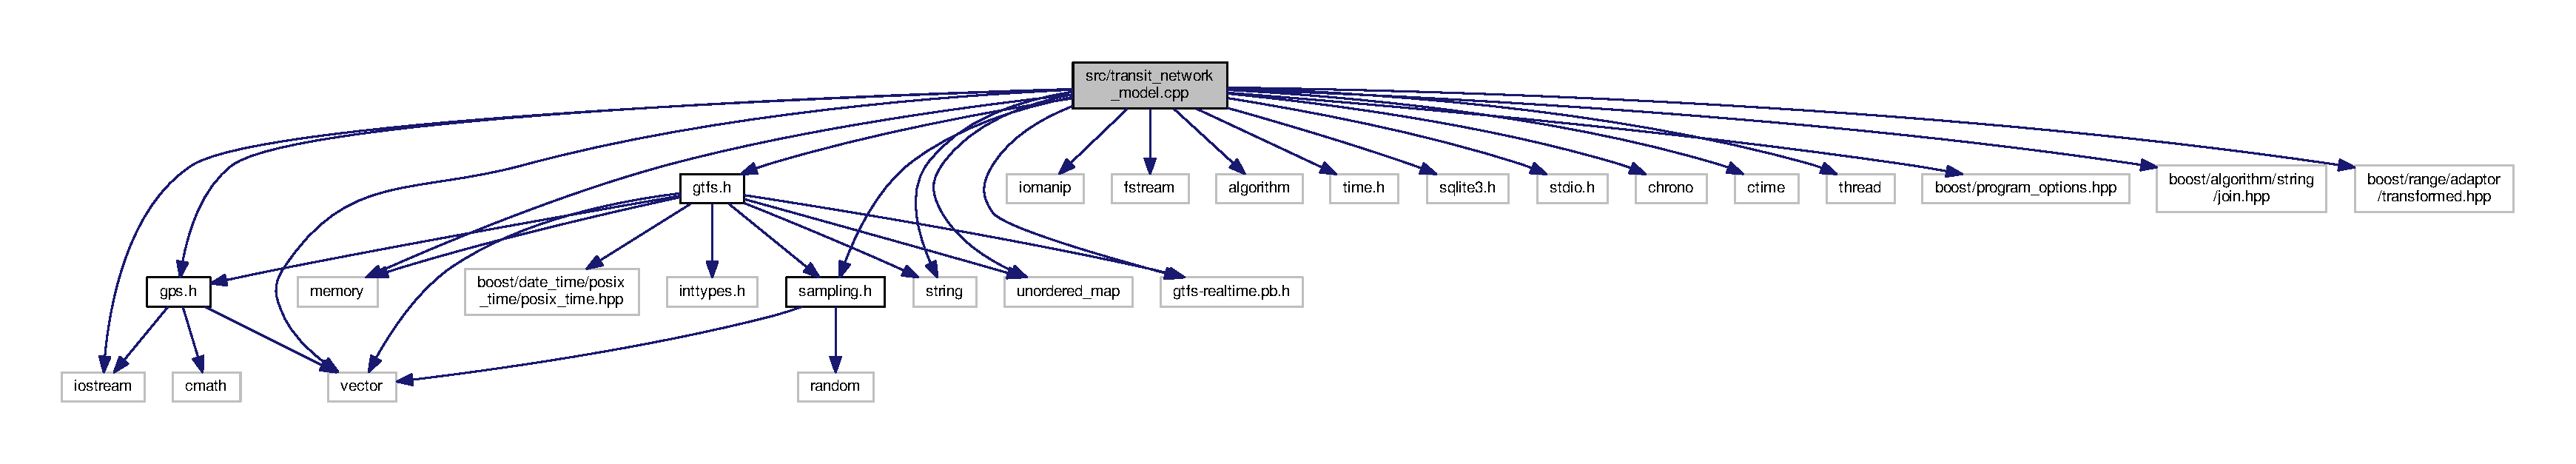
\includegraphics[width=350pt]{transit__network__model_8cpp__incl}
\end{center}
\end{figure}
\subsection*{Functions}
\begin{DoxyCompactItemize}
\item 
int \hyperlink{transit__network__model_8cpp_a0ddf1224851353fc92bfbff6f499fa97}{main} (int argc, char $\ast$argv\mbox{[}$\,$\mbox{]})
\end{DoxyCompactItemize}


\subsection{Detailed Description}
\begin{DoxyAuthor}{Author}
Tom Elliott \href{mailto:tom.elliott@auckland.ac.nz}{\tt tom.\+elliott@auckland.\+ac.\+nz} 
\end{DoxyAuthor}
\begin{DoxyVersion}{Version}
0.\+0.\+1 
\end{DoxyVersion}


\subsection{Function Documentation}
\index{transit\+\_\+network\+\_\+model.\+cpp@{transit\+\_\+network\+\_\+model.\+cpp}!main@{main}}
\index{main@{main}!transit\+\_\+network\+\_\+model.\+cpp@{transit\+\_\+network\+\_\+model.\+cpp}}
\subsubsection[{\texorpdfstring{main(int argc, char $\ast$argv[])}{main(int argc, char *argv[])}}]{\setlength{\rightskip}{0pt plus 5cm}int main (
\begin{DoxyParamCaption}
\item[{int}]{argc, }
\item[{char $\ast$}]{argv\mbox{[}$\,$\mbox{]}}
\end{DoxyParamCaption}
)}\hypertarget{transit__network__model_8cpp_a0ddf1224851353fc92bfbff6f499fa97}{}\label{transit__network__model_8cpp_a0ddf1224851353fc92bfbff6f499fa97}
Transit Network Model\+: a realtime model running indefinitely (while (true) \{ ... \})

Cycles through latest vehicles in the Realtime Feed, and updates/creates accordingly.


\begin{DoxyParams}{Parameters}
{\em argc} & number of command line arguments \\
\hline
{\em argv} & argument vector \\
\hline
\end{DoxyParams}
\begin{DoxyReturn}{Returns}
int 0 (although this will never happen because of the while forever loop) 
\end{DoxyReturn}

%--- End generated contents ---

% Index
\backmatter
\newpage
\phantomsection
\clearemptydoublepage
\addcontentsline{toc}{chapter}{Index}
\printindex

\end{document}
